\documentclass[A4,12pt]{article}
\usepackage{geometry}
\usepackage{multicol}
\usepackage{lipsum}
\usepackage{changepage}
\usepackage{graphicx}
\graphicspath{  }
\usepackage{booktabs}
\usepackage{cite}
\usepackage{float}
\usepackage{hyperref}
\usepackage[font={small,it}]{caption}
\usepackage[english]{babel}
\usepackage{fancyhdr}

\setlength{\headheight}{15pt}

\pagestyle{fancy}
\fancyhf{}
\lhead{\textbf{Version:} 2.0  \textbf{Revision:} 10/27/17}
\rhead{\thepage}
\lfoot{Sam Penders}
\rfoot{\textit{Mu2e: University of Minnesota}}

\renewcommand{\footrulewidth}{1pt}

\begin{document}

\begin{titlepage}
	\centering
	
\includegraphics[width=0.5\textwidth]{mu2e_logo_oval.png}\par\vspace{2cm}
	{\scshape\LARGE CO$_2$ Leak Testing of Straws \\
		Standard Operating Procedure\par}
	\vspace{3cm}
	{\Large Sam Penders\par}
	\vspace{3cm}
	{\large University of Minnesota\par}
 	\vspace{.5cm}
	{\large October 27, 2017\par}
	% Bottom of the page
	\vfill
	{\href{mailto:pende061@physics.umn.edu}{\tt{pende061@physics.umn.edu}}\par}
\end{titlepage}

\clearpage
\setcounter{page}{1}

\newenvironment{myitemize} %adjust item spacing in lists to make smaller
{ \begin{itemize}
    \setlength{\itemsep}{4pt}
    \setlength{\parskip}{0pt}
    \setlength{\parsep}{0pt}     }
{ \end{itemize}                  } 

\section{Goal}
All Mylar straws in the Mu2e electron tracker panels will be inflated with a mix of argon gas and CO$_2$ during the run of the experiment. Thus, our goal is to determine the leak rate of each straw before panel installation, as well as identify straws that are damaged. We strive to do this in a safe, efficient, and reproducible manner.

%-----------------------------------------------
%	EQUIPMENT
%-----------------------------------------------

\section{Equipment Used}
\begin{multicols}{2}
\begin{myitemize}
	\item Pallet with Mylar straws
	\item CO$_2$ tank with regulator attached
	\item N$_2$ tank with regulator attached
	\item CO$_2$ pressure gauge and flow meter with hose 
	\item Vacuum grease
	\item Straw endpiece hose plugs
	\item Leak test chambers
	\item Plastic straw loading tubes
	\item Magnetic grabber
	\item Arduino Unos connected to leak chambers and computer
	\item Isopropyl alcohol and paper towels
	\item Form--fitting nitrile gloves
\end{myitemize}
\end{multicols}

%-----------------------------------------------
%	RISKS AND DANGERS
%-----------------------------------------------

\section{Risks and Dangers}
There is an inherent danger when working with pressurized gases. Because the N$_2$ and CO$_2$ tanks are pressurized to a maximum of 2500 psi, an uncontrolled discharge of gas from the cylinders would effectively make the cylinders into rockets. This could happen in a cylinder is knocked over and the gas cylinder valve or regulator valve gets damaged. For this reason, compressed gas chambers are harnessed to the wall by a chain. The regulator over the exit valve limits the pressure of gas released from the chamber. To prevent accidental tipping of the cylinders, only a trained supervisor should ever move cylinders or adjust regulator pressure. 

High levels of CO$_2$ in the air can make a person feel dizzy. To CO$_2$ levels from getting high, the lab has a good ventilation system. Make sure that you can hear the sound of fans from the laboratory ventilation system when working with the CO$_2$. If you do feel dizzy, close the CO$_2$ tank valve and step outside for a few minutes. Always close the gas tanks when not in use.

Care must be taken when cleaning with isopropyl alcohol. Contact with skin can cause irritation, so nitrile gloves should be worn at all times. If alcohol gets on skin, it should be washed off with soap and water. If alcohol gets in your eyes, they should be rinsed in the eye wash for several minutes. Then, go to a doctor.


\newpage

\section{Leak Testing Procedure}

\subsection{Setup}

\begin{enumerate}
	\item Put on nitrile gloves that fit snuggly. These must be worn at all times when handling straws.
	\item Check that the regulator is attached to CO$_2$ tank. Do not touch center regulator knob. Open both the gas cylinder and regulator exit valve completely. (Figure \ref{co2tank}) If these are only partially opened, gas may leak from the valve.   
	\item Check cylinder pressure. If below 200 psi, stop using cylinder immediately. If below 500 psi, have Dan order a new cylinder.
	\item Adjust flow meter on near pressure gauge to 10 scfh. Cover end of CO$_2$ nozzle with finger and confirm that the pressure on near pressure gauge reads $14.7 \pm 0.1$ psi. If not, consult a supervisor.
\end{enumerate}

\begin{figure}
	\center
	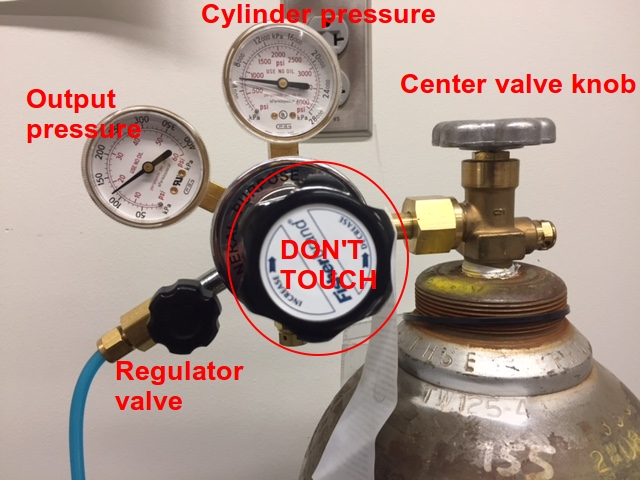
\includegraphics[scale=0.5]{co2tank}
	\caption{CO$_2$ tank with regulator attached. The regulator adjustment knob in the center should not be adjusted. The N$_2$ tank regulator is identical.} \label{co2tank}
\end{figure}

\subsection{Emptying Leak Chamber}
	\begin{enumerate}
		\item On computer, go to the window with the leak test program running (if the program is open and running. If not, proceed to section \ref{performing test}). If a straw passed or failed the test, select the $j^{th}$ chamber (where $j$ is the chamber number, e.g. 1) by entering: \texttt{chj} 
		
Then, enter: \texttt{empty}

The $j^{th}$ leak chamber is now ready to be physically emptied. \label{empty1}

	\item With chamber emptied in computer, open white valve lever on leak chamber. Gently slide magnetic stick into chamber until connection with steel nut is made. Pull tube out of chamber.
	\item Carefully slide tube off of straw and put tube back into leak chamber (leaving the last inch of it sticking out). 
	\item Pull both hose plugs out of straw. Pick up straw by gently pulling straw hoses taut. Put straw back into spot on pallet. \label{emptylast}
	\item Repeat steps \ref{empty1}--\ref{emptylast} until all finished straws are out of chamber.
	\item Start performing next leak test.
	
\end{enumerate}

\subsection{Performing Test} \label{performing test}
	\begin{enumerate}
		\item On N$_2$ tank, open center and regulator valves by a full turn. Make sure N$_2$ valve is closed on each leak chamber.
		\item Insert nozzle into straw endpiece hose and let flush for 10 seconds. Meanwhile, apply a dab of vacuum grease to a hose plug, and plug hose on side opposite to CO$_2$ nozzle. \label{1}
		\item Apply dab of vacuum grease to another plug. On CO$_2$ hose side of straw, pinch endpiece hose with pliers and remove CO$_2$ hose. While continuing to pinch hose, insert plug into straw hose.
		\item Grab hoses on both sides of straw, apply slight tension to straw, and carefully lift straw out of pallet. Slide straw into plastic tube.
		\item Check that leak test chamber is empty, and slide tube into chamber, with the metal nut side of tube going in last. 
		\item With straw in chamber and the chamber open, open black N$_2$ valve lever on chamber so it will flush. \label{flush}
		\item Repeat steps \ref{1}--\ref{flush} until each chamber contains a straw. Each time a straw goes in a chamber, close the black N$_2$ valve lever on the previously loaded chamber, and then close the white lever on that same chamber. Then, open black N$_2$ valve lever on the chamber you just loaded while keeping straw loading valve open, as before.
\end{enumerate}

	

\subsection{Cleanup}
	\begin{enumerate}
		\item Make sure that N$_2$ and CO$_2$ cylinder and regulator valves are closed.
		\item Put any extra straw endpiece hose plugs back into their container.
		\item Wipe any clean any vacuum grease off of work surface with alcohol and paper towel.
		\item Throw away gloves|they likely have vacuum grease on them.
	\end{enumerate}



\section{Troubleshooting}

\begin{itemize}
	\item {\bf Problem:} One of the chambers isn't taking data.
		\begin{adjustwidth}{1cm}{}
		{\bf Solution:} Make sure that the sensor cable is attached to the chamber, and is plugged securely into its Arduino port. If this doesn't work, sometimes the CO$_2$ level offset can be initially to low in the chamber. Open the straw loading valve and exhale for about half a second into chamber, then close valve. If this does not help, unplug Arduino from power supply for a minute. Then replug and try again. If the problem persists, ask for help.
		\end{adjustwidth}
	
	\item {\bf Problem:} I accidentally scanned the wrong straw for a chamber.
		\begin{adjustwidth}{1cm}{}
		{\bf Solution:} Empty the chamber in the program. Ask a manager to delete the incorrectly named file. Re-enter the correct straw in the leak test program.
		\end{adjustwidth}
\newpage		
\item {\bf Problem:} A straw is epoxied at the endpiece to the pallet, so I can't remove it.
		\begin{adjustwidth}{1cm}{}
		{\bf Solution:} Carefully try to peel stuck end off of plastic. If it looks okay, leak test it as usual. If it is obviously damaged, cut damaged end off of straw and give to epoxy station to re-epoxy and endpiece in.
		\end{adjustwidth}
		
\item {\bf Problem:} A straw is stuck in the chamber.
		\begin{adjustwidth}{1cm}{}
		{\bf Solution:} Unplug sensor cable from chamber, and slide entire chamber off of rack. With the straw loading valve open and hold over valve, tip chamber upside down and try to shake straw out. If this doesn't work, try to grab onto the straw with claw grabber. If this doesn't work, consult manager.
		\end{adjustwidth}
		

\end{itemize}











\end{document}
